\chapter{Implementation}
\label{cha:implementation}

In this chapter, we turn our attention to the technical implementation of the concept. In particular, we will look at programming
peculiarities, as well as the structure of the extension, the infrastructure of the backend and problems that occurred during the implementation.

\section{Web Extension}
We begin with the implementation of the web extension. To better illustrate the components and implementation decisions we divided this section
in five different subsections each describing important implementation aspects. In section \ref{sec:frameworks} we discuss the frameworks
and libraries which are required in order to implement the extension. Following up in section \ref{sec:bl} we explain the business logic 
the extension and look at implementation details. In section \ref{sec:ui} we show the user interface and explain how a user can interact with
the application. In the final section \ref{sec:lim} we show limitations of the application in its infrastructure and its design. Moreover, we give
an outlook on how the extension can be improved in future iterations.
\subsection{Frameworks}
\label{sec:frameworks}
The most important framework for this application is \emph{TensorFlow.js} \cite{tensorflowJs}.
TensorFlow.js is a powerful library used for machine learning tasks in web-based applications.
It enables the deployment and execution of trained machine learning models directly in web browsers.
By leveraging the capabilities of JavaScript, TensorFlow.js empowers developers to build and deploy AI-powered
applications that can run natively in the browser environment, without the need for additional server-side infrastructure.

One of the key features of TensorFlow.js is its ability to leverage the computational power of modern web browsers and GPUs
to perform complex computations required for training and inference. By utilizing WebGL and WebGPU technologies, TensorFlow.js
harnesses the parallel processing capabilities of these hardware resources, enabling efficient and high-performance execution
of machine learning models. This high performance and the ability to run TensorFlow models in the browser is the key feature why it is
used in our extension. Without TesnsorFlow.js the creation of this application would not be possible.

For the user interface we use \emph{Vue.js} \cite{vuejs} which is a versatile JavaScript framework widely used for building user
interfaces and single-page applications. It provides developers with a robust and intuitive tool set for creating interactive
and dynamic web applications. Vue.js follows a component-based architecture, allowing developers to encapsulate reusable
UI components and compose them to build complex user interfaces.

Additionally, we use \emph{Vuetify} \cite{vuetify} which is a popular open-source UI component library for Vue.js, designed
to facilitate the development of responsive and visually appealing web applications. It offers a comprehensive set of reusable
components and ready-to-use design patterns. Vuetify follows Material Design principles, which provide consistent and visually
appealing UI elements. Vue.js and Vuetify build the basis for any user interface in this application as it is simple to use, and 
the UI components are already used by multiple professional websites.

A web extension is a complex application as it is composed of multiple small applications which communicate through the browsers' API. This
is especially complicated when dealing with large and complex extensions. Therefore, we use \emph{Vite} \cite{vite} as a bundler
for our JavaScript and Vue.js applications. Vite is a fast and lightweight build tool for modern web applications. It provides
a streamlined development experience by leveraging native ES module imports in the browser. Vite eliminates the need for
bundling during development, allowing for near-instantaneous hot module replacement (HMR) and faster startup times. Using Vite as a bundler
for our web extension enables faster development and better testing capabilities.

The use of these frameworks is crucial for the implementation of our web extension as they provide the technologies and the speed to create
this kind of project in the given timespan. 
\subsection{Business Logic}
\label{sec:bl}
The business logic of the web extension is located in the background page of the extension. 
The TensorFlow model gets loaded in \emph{Model.js} component of the extension which is shown in Fig-\ref{fig:Model}.
\begin{figure}[ht!]
  \begin{lstlisting}[language=JavaScript]
// Model.js
import * as tf from "@tensorflow/tfjs";
/*
The component which is in charge of loading the TensorFlowJs model 
and providing the predict function which can be used to predict 
a given feature vector.
*/ 
const Model = (async () => {
  // First determine the resource URL to the model.json file which includes all the metadata to the given model
  const MODEL_URI = browser.runtime.getURL("model/model.json");
  // Then we pass the URI into the tensorflow function which downloads the model structure and the model weights and stores them into memory
  const model = await tf.loadLayersModel(MODEL_URI);
  return {
    predict(features) {
      return model.predict(features);
    },
  };
})();

export { Model };
  \end{lstlisting}
  \caption{This listing shows the loading of the TensorFlow model. The model can only be loaded asynchronously and cannot predict any 
  requests unless it is loaded completely. The model object gets exported for other components of the background page.}
  \label{fig:Model}
\end{figure}

In that component we first import TensorFlow and then locate the path of the \emph{model.json}. Note that this component is asynchronous
which is problematic because the callback to block web requests is synchronous. We await the model and return an object with a predict function.
This function takes a TensorFlow vector as a parameter and passes it to the awaited model. After that it returns the prediction of the model.

\begin{figure}[ht!]
  \begin{lstlisting}[language=JavaScript]
// RequestBlocker.js
import { Model } from "./Model";
import { FeatureExtractor } from "./FeatureExtractor";
import { StatsListener } from "./StatsListener";
/*
The definition of the component which is in charge of feeding the
feature vector in the TensorFlowJs model.
*/
const RequestBlocker = (async () => {
  let model = await Model;
  return {
    check(request) {
      let encoding = FeatureExtractor.encode(request);

      let result = model.predict(encoding);

      const values = result.dataSync();
      const arr = Array.from(values);

      return { predict: arr[0], blocked: arr[0] >= StatsListener.getRate() };
    },
  };
})();

export { RequestBlocker };
\end{lstlisting}
\caption{The \emph{RequestBlocker} component is in charge of creating the feature vector using the \emph{FeatureExtractor} and passing the 
result into the \emph{Model}. After that, it returns the prediction score to the callee of the \emph{check} function.}
\label{fig:blocker}
\end{figure}
The Model component is primarily used in the \emph{RequestBlocker} component which is illustrated in Fig-\ref{fig:blocker}. The RequestBlocker
component is in charge of blocking certain requests exceeding the user set threshold. It does that by awaiting the Model component so that 
it can be used synchronous, and it returns a check method which takes a request JSON object as a parameter. The \emph{FeatureExtractor}
is called to encode the request into a numeric tensor representation. This encoded feature vector gets passed to the model which returns
a tensor with prediction value. In order to load the data of the tensor the \emph{dataSync} method is called. After that, the \emph{check}
method returns a JSON object with the prediction score and whether a request should be blocked or not. This is done by comparing the model result
with the user set threshold in the \emph{StatsListener} component.
\begin{figure}[ht!]
\begin{lstlisting}[language=JavaScript]
// EventListener.js
const EventListener = (async () => {
  const urlFilter = { urls: ["http://*/*", "https://*/*"] };
  const blocker = await RequestBlocker;
// ...
    browser.webRequest.onBeforeSendHeaders.addListener(
      // Here we add an EventListener to the onBeforeSendHeaders event.
       (details) => {
        setRequest(details.requestId, {
          requestHeaders: details.requestHeaders,
        });
        // We check whether the request is concidered a tracking request by passing all available information into the blocker component
        let result = blocker.check(details);
        setRequest(details.requestId, {
          ...result,
        });
        pushToQueue(details.requestId);
        // We send a blocking signal whenever the result is true and the blocking setting is active
        return { cancel: result.blocked && StatsListener.isActive() };
      },
      urlFilter,
      ["requestHeaders", "extraHeaders", "blocking"]
    );
// ...
})();
\end{lstlisting}
\caption{This figure shows the code for the web request blocking inside the web extension. The details get passed to the blocker component 
  which is in charge of calling the ML model to determine weather a request should be blocked. A request can only be blocked when the blocking is
  activated in the UI. This is indicated with the \emph{isActive} call on the \emph{StatsListener}.
}
\end{figure}

The RequestBlocker component is used in the \emph{EventListener} component. In that component we await the asynchronous RequestBlocker to 
use later it synchronously in the callback of the \emph{onBeforeSendHeaders} event which is provided by the browser API. In that callback there 
some functionality to store the requests to later display them in the user interface. The \emph{check} method gets called with the request details
provided by the browser API. To cancel a request using the browser API it is important to return a JSON object with a cancel field set
to true. In this implementation we pass the model result and check whether the user has activated the blocking of requests.

Note that this is just a small excerpt of the code to demonstrate the usage of the TensorFlow model in this kind of environment. The whole background page
is also in charge of collecting requests to later display them and to order the requests to the tabs they got executed in. Furthermore, it is 
responsible to send the collected data to the storage from which the frontend can retrieve it. The full source code of this web extension is open-source
and listed on GitHub \cite{trackingDetector}.
\subsection{User Interface}
\label{sec:ui}
In this section we turn our focus on the user interface which is the part of the application visible to the end user. Most of the user 
interface for this application is located in the popup of the web extension. As mentioned before the user interface is a Vue.js application
using Vuetify for the styling and the general components.


\begin{figure}[ht!]  
  \centering
  \begin{subfigure}[b]{.30\textwidth}
      \centering
      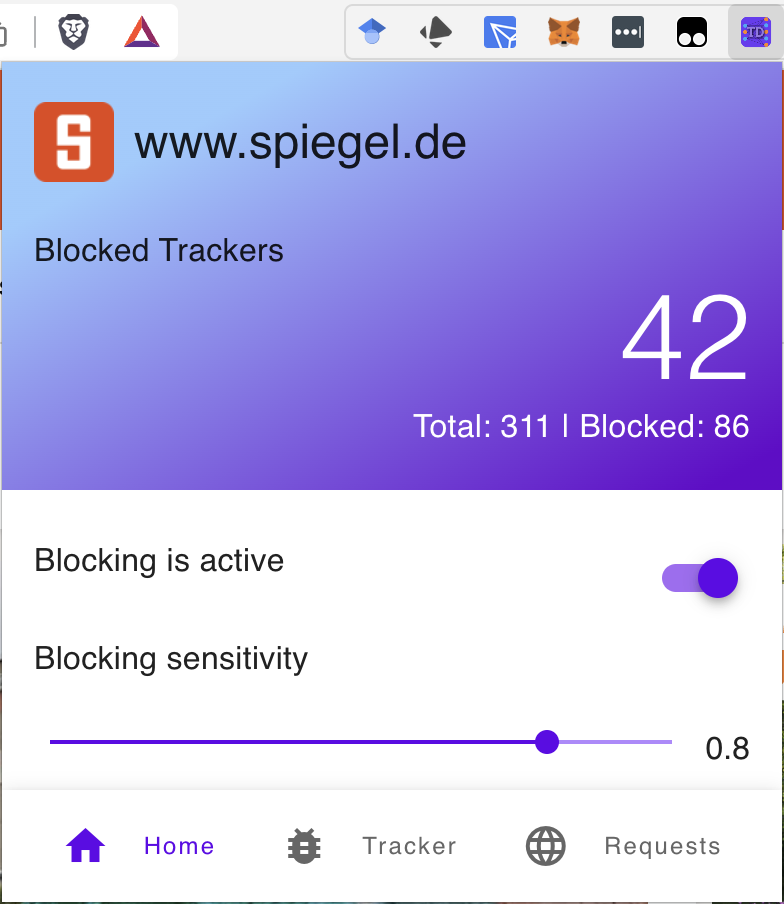
\includegraphics[width=\linewidth ]{images/Home.png}
      \caption{The \emph{Home} page of the popup gives general information about the current visited page. It shows the amount
      of identified trackers, the amount of total requests and the amount of blocked requests. It also introduces controls
    for the user to regulate the blocking sensitivity and whether a request should be blocked at all.}
      \label{fig:Home}
  \end{subfigure}
  \hfill
  \begin{subfigure}[b]{.30\textwidth}
      \centering
      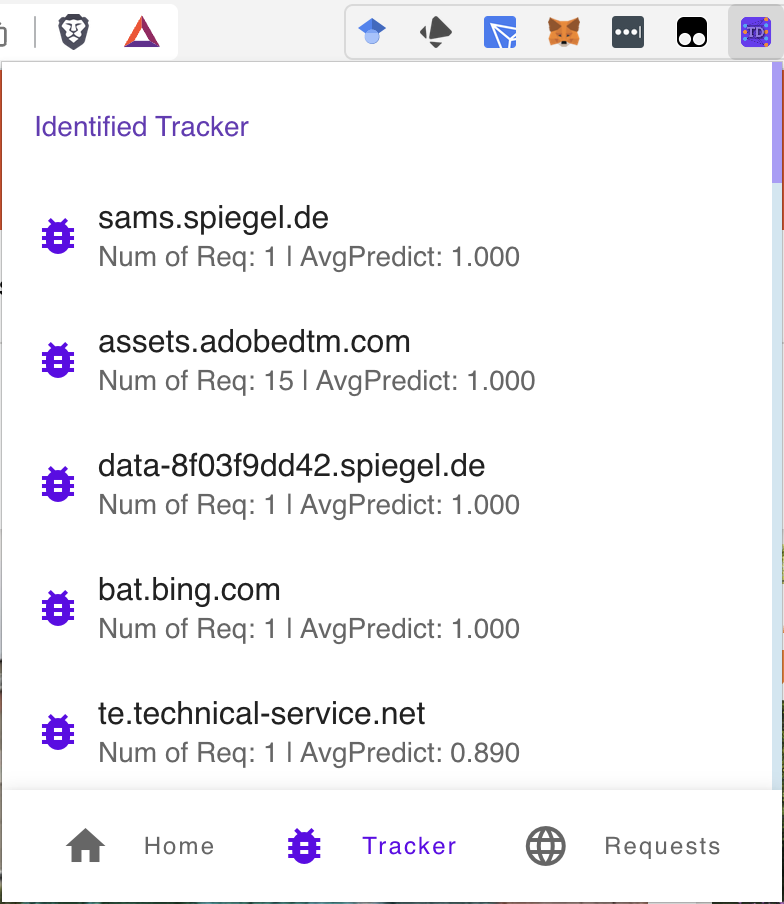
\includegraphics[width=\linewidth, keepaspectratio]{images/Tracker.png}
      \caption{The \emph{Tracker} page shows the identified trackers on a given page. It lists the tracker domain and 
      the number of requests that the currently visited webpage wanted to perform against that domain inside a list. Furthermore, it shows
    the average prediction of the model for all requests that were sent to that domain.}
      \label{fig:Tracker}
  \end{subfigure}
  \hfill
  \begin{subfigure}[b]{.30\textwidth}
      \centering
      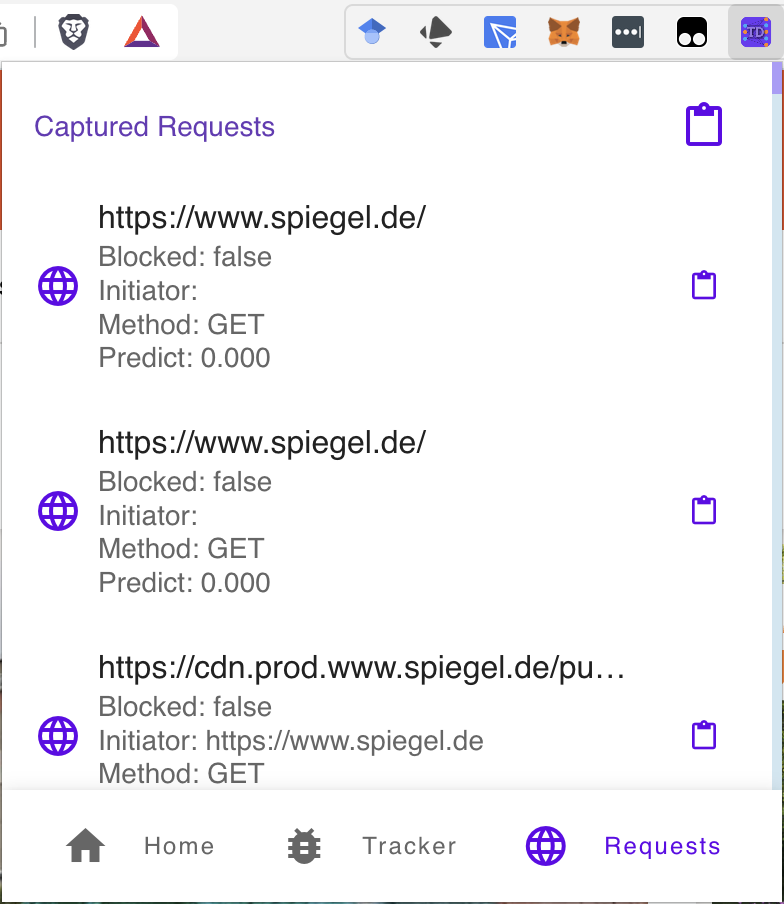
\includegraphics[width=\linewidth, keepaspectratio]{images/Requests.png}
      \caption{The \emph{Request} page shows all requests performed on the currently visited webpage. It also provides a button to export
      requests as JSON format into the clipboard. In that view the requested URL, the model prediction, whether a request has been blocked,  the request initiator and the request 
    method is shown for each request.}
      \label{fig:Requests}
  \end{subfigure}
  \caption{This figure shows the user interface of the popup. The user interface consists of three different pages which
  serve different purposes.}
  \label{fig:popup}
\end{figure}  

The most important user interface regarding the usage of the application is the extension popup which is shown in Fig-\ref{fig:popup}.
This user interface is in charge of communicating the state of the application and the identified trackers on the currently visited 
website to the end user. Moreover, it is important that the popup is simple to use and expressive regarding information about the trackers identified.
To solve this we implemented our popup to consist of three different pages which all display different information about the currently
visited website. For the navigation between the pages we used the \emph{BottonNavigation} component of Vuetify.

The initial when opening the popup view is the \emph{Home} page which is shown in Fig-\ref{fig:Home}. This page
allows the user to switch the blocking state and to toggle the blocking sensitivity. Whenever a setting is changed the current loaded
browser tab gets reloaded. Additionally, this page displays brief information about the tracking behavior of the current visited website.
It shows the URL, the favicon of that page, the amount of identified trackers and the total and blocked requests that website performed. 
All the user interface for this page is using the Vuetify component system with some CSS modifications for the gradient and the layout.

The \emph{Tracker} page in Fig-\ref{fig:Tracker} displays more information about the identified trackers on the currently
visited website. The page includes a list of items with each item representing a tracker domain identified. The item displays the amount of
request that should go to that domain and the average prediction score of the model. As we use an ML model the scores could vary if some parameter
of the feature vector changes. Therefore, we calculate and show the average for each tracker listed in the list view.

Moreover, the \emph{Requests} page, which is displayed in Fig-\ref{fig:Requests}, shows all request executed on the currently active tab. This information is condensed into the URL 
whether a request was blocked, the request initiator, the request method and prediction score of the model. Additionally, there are buttons to store all or each request as JSON into the clipboard.
This JSON string includes all the information collected by the background page. This feature is mainly for debugging and data analysis.

There is an option page under development which should create a seamless integration into the designed backend.
\begin{figure}
  \begin{center}
    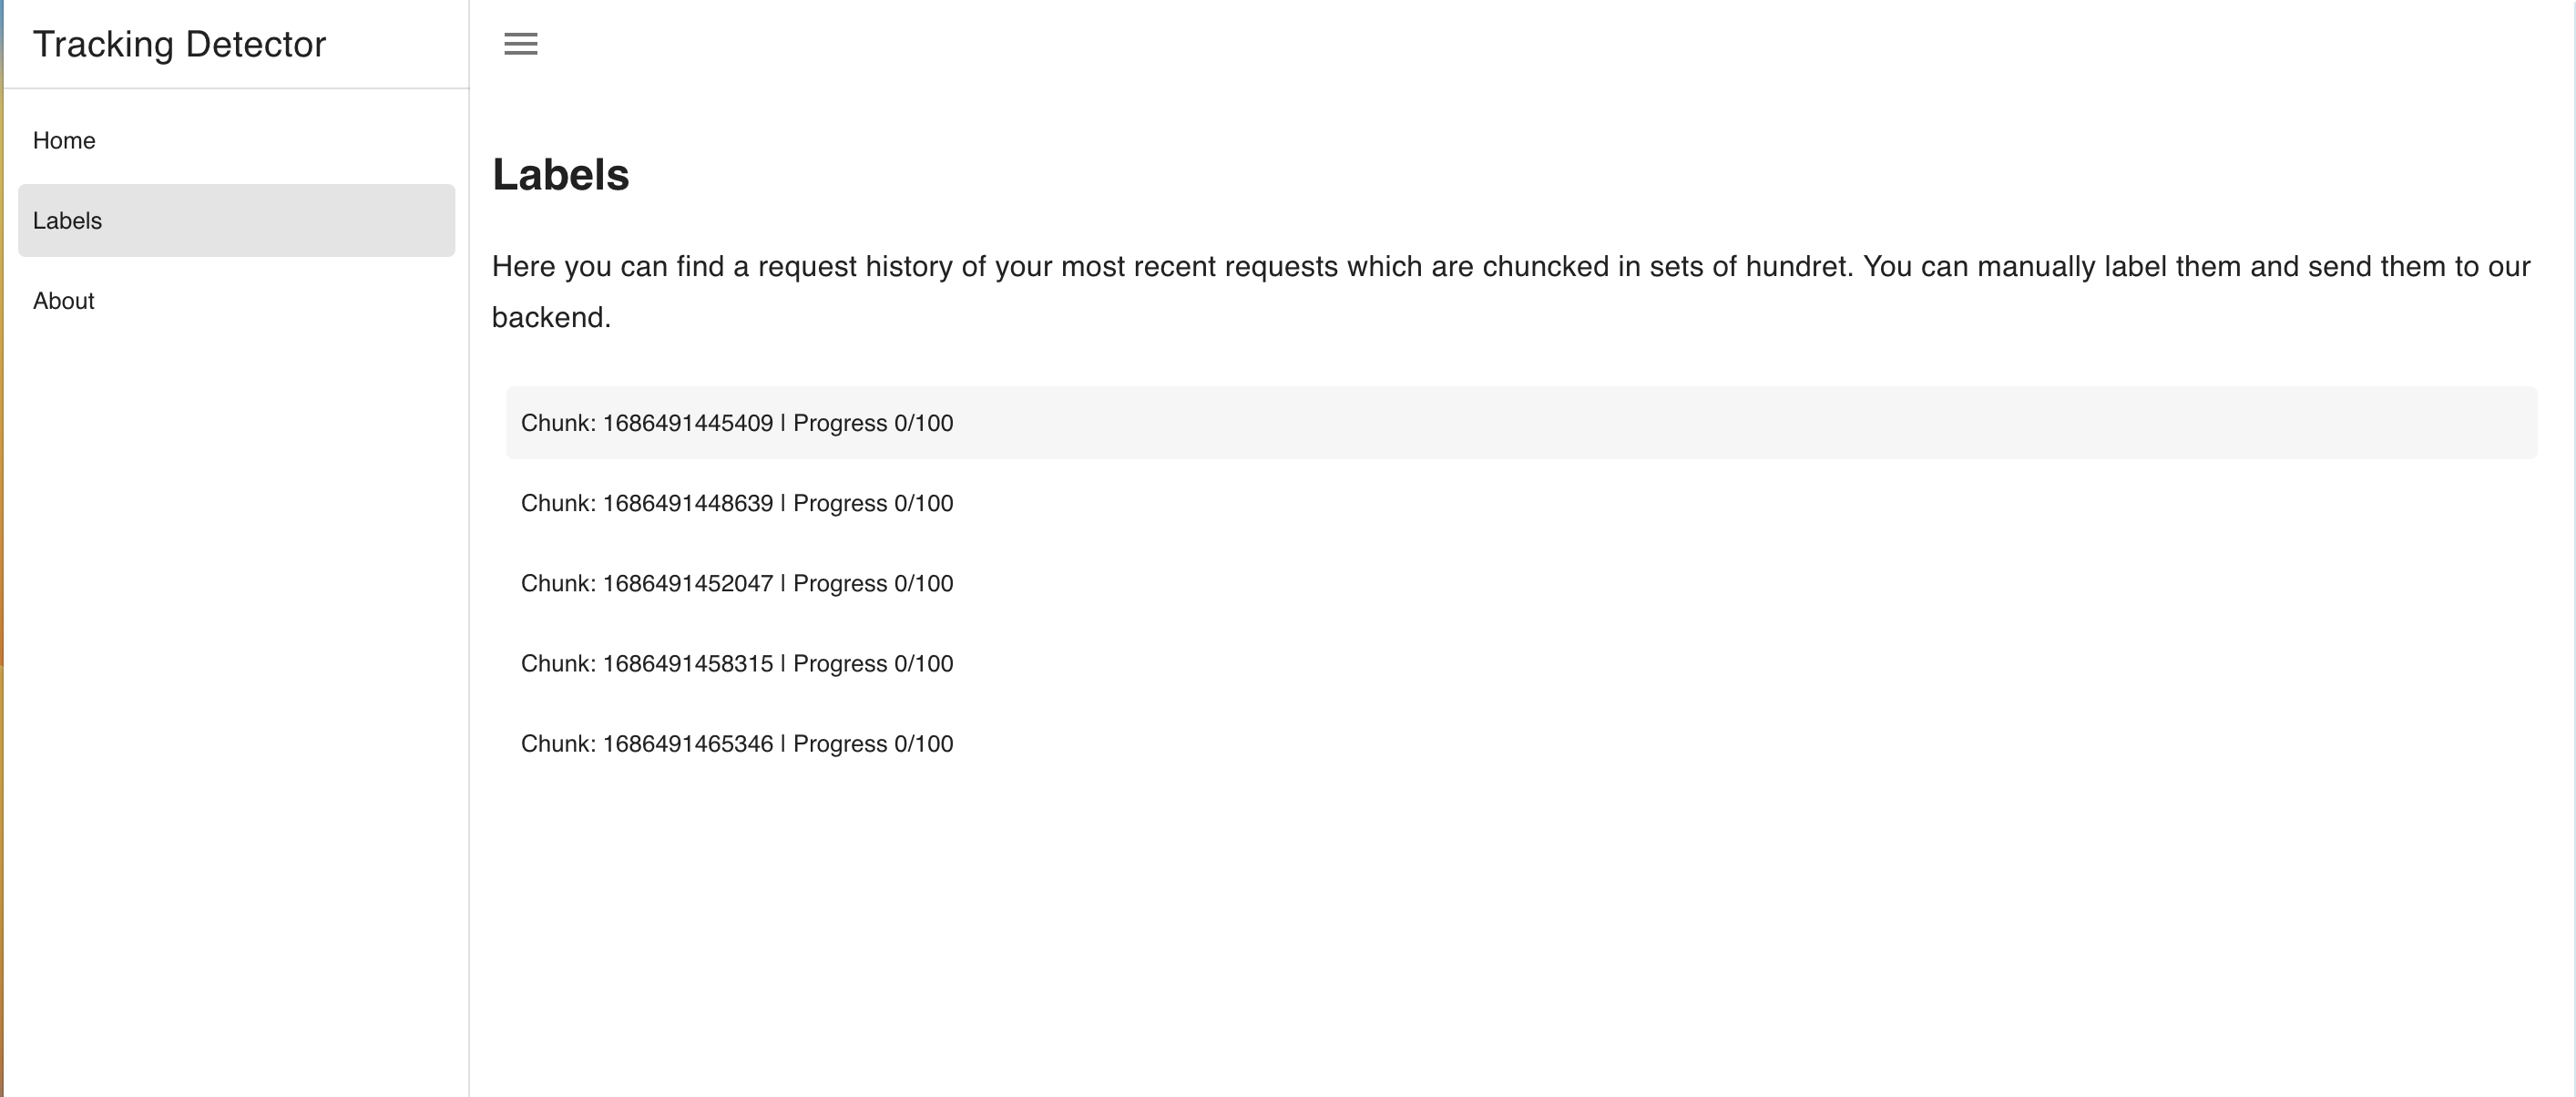
\includegraphics[width=0.95\textwidth]{images/LabelsPage.png}
  \end{center}
  \caption{This figure shows the options page of the \emph{Tracking Detector} extension. In specific the \emph{Labels} page is shown which 
  is used to show chunks of request data which the user can label by itself and send to the training backend.}
  \label{fig:LabelsPage}
\end{figure}
The option page is divided into three different pages which can be navigated through the navigation drawer provided by Vuetify. The landing 
page gives a brief introduction on how this application works and how the user can participate to create a better ground truth for the ML models.
The \emph{About} page list general information on how to cite this work and the authors of this application. The \emph{Labels} page in Fig-\ref{fig:LabelsPage} is responsible
for showing the chunks the user browsed through and allows labeling each request
individually. The chunks come from the background page and get loaded into the options page. Each chunk consists of 100 requests in JSON format 
which can be labeled in the browser. 
\begin{figure}
  \begin{center}
    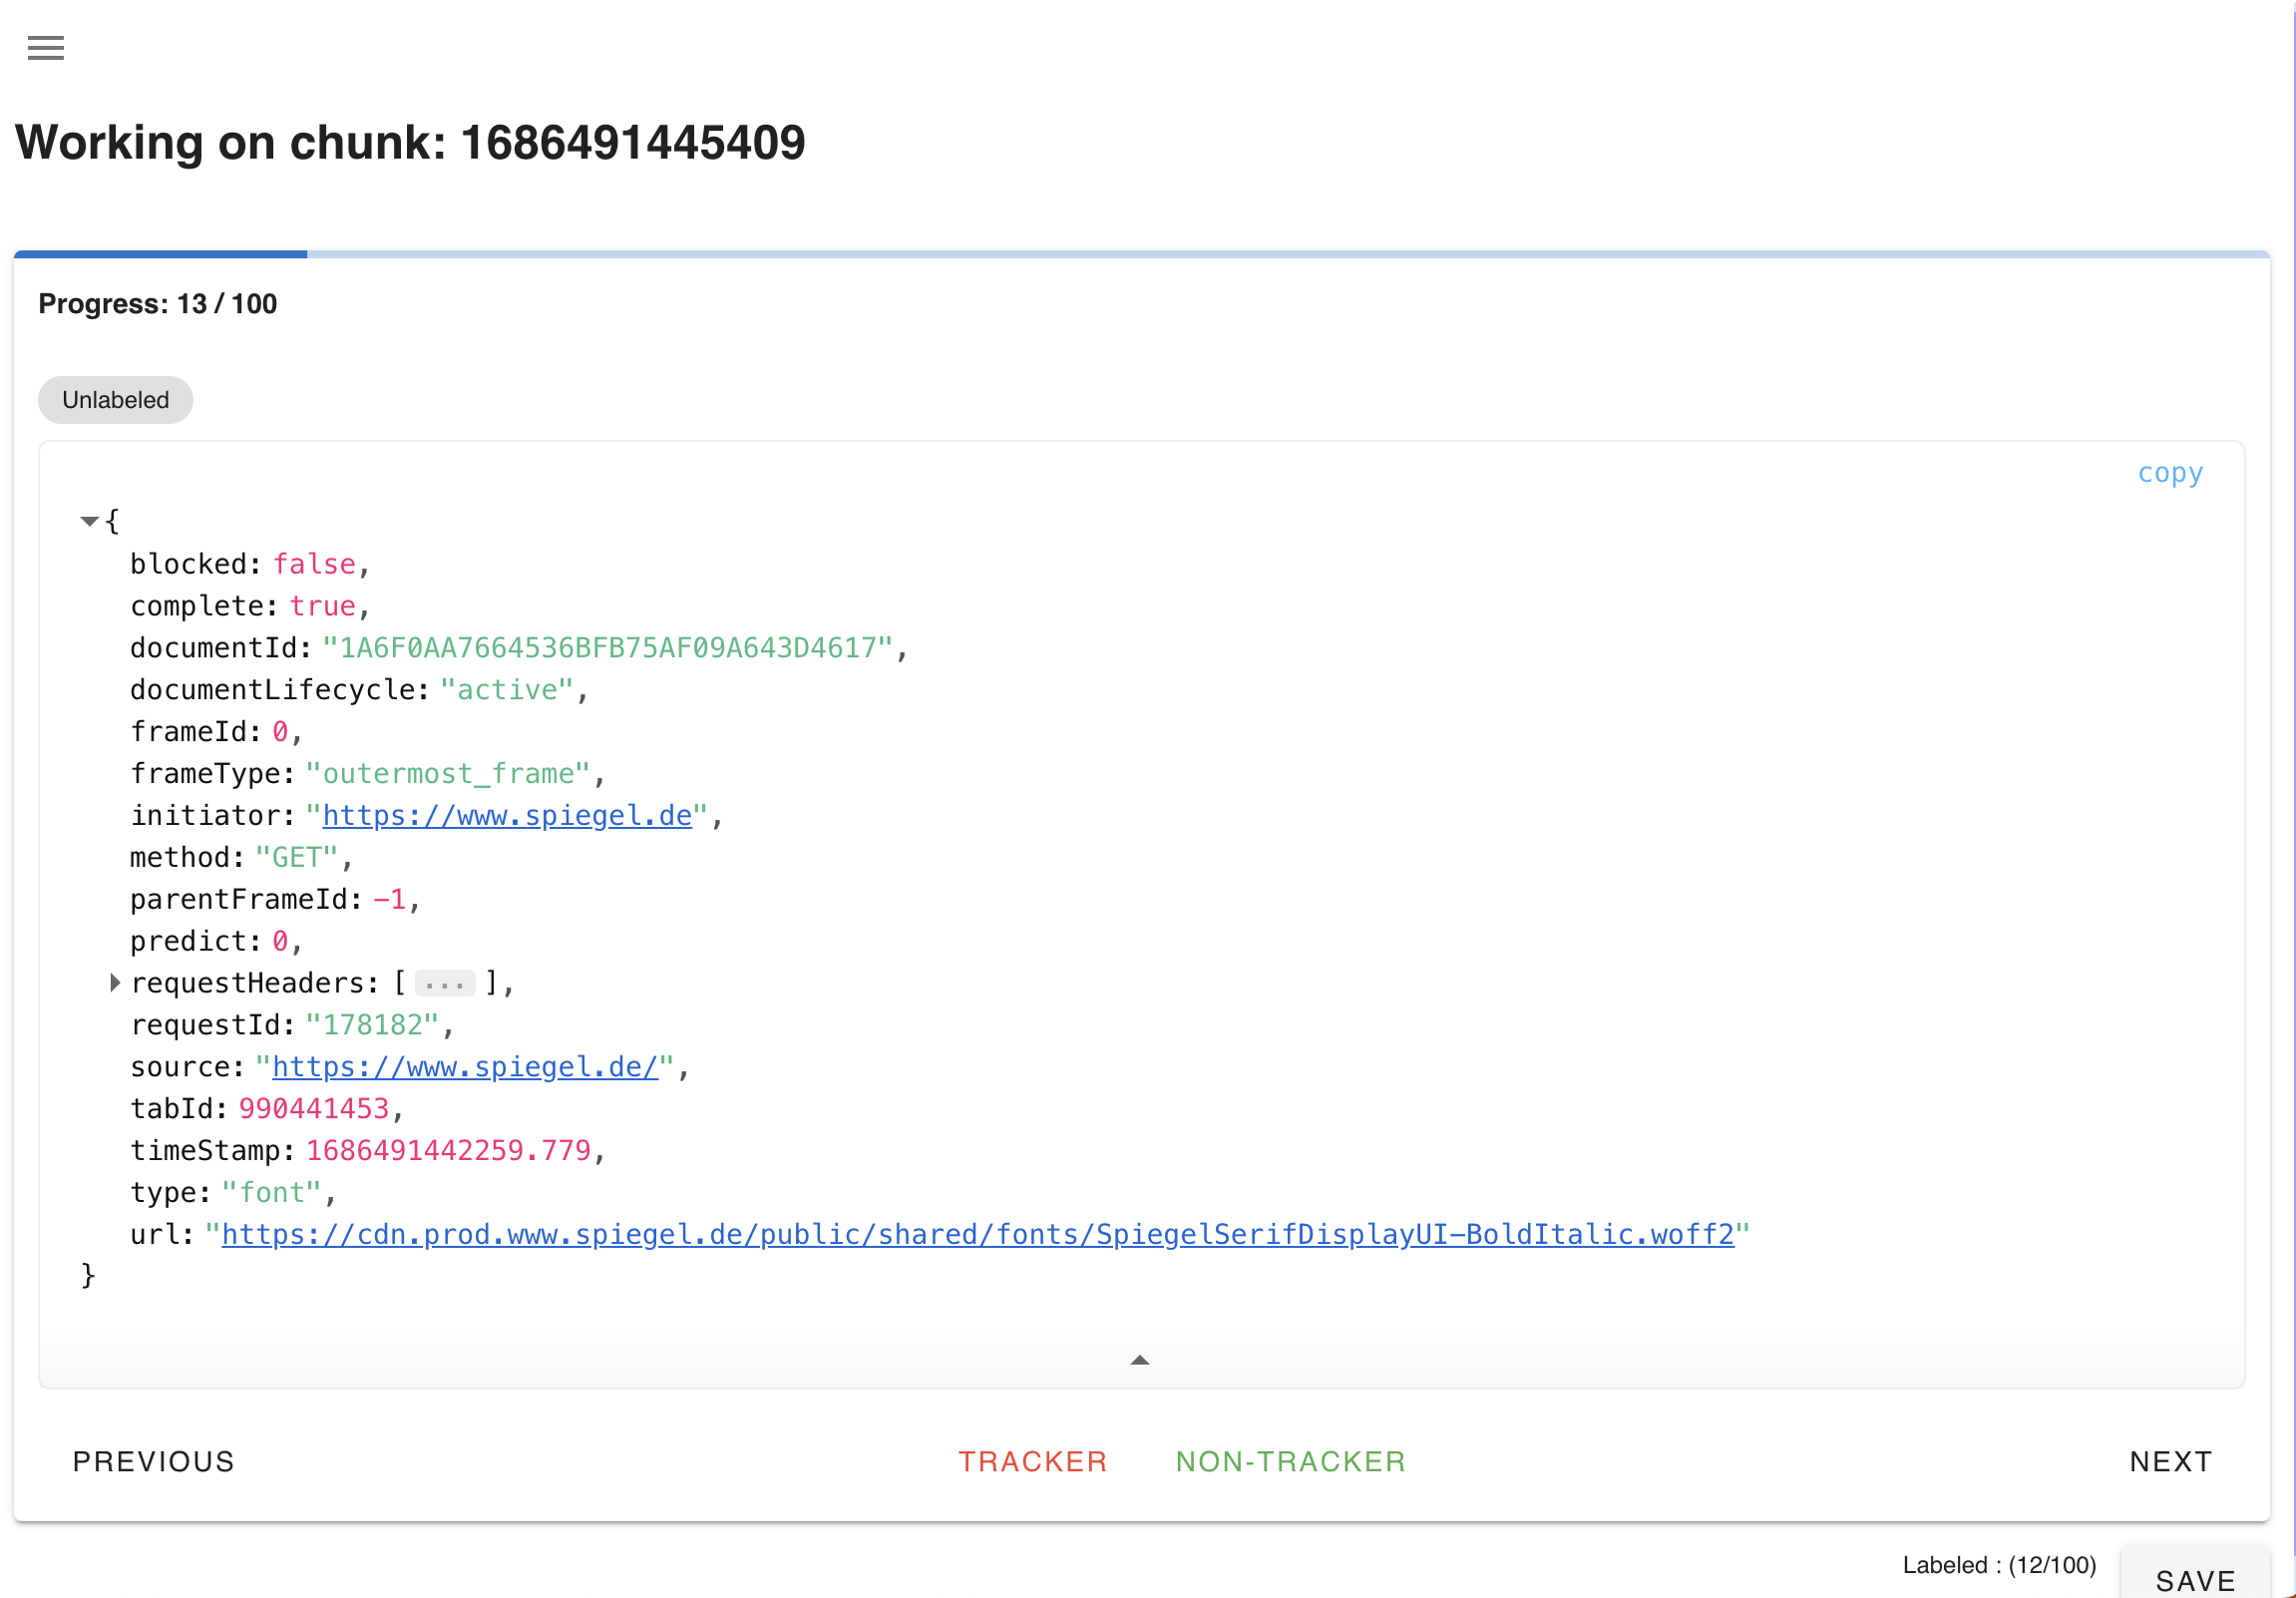
\includegraphics[width=0.95\textwidth]{images/Labeling.png}
  \end{center}
  \caption{This figure shows the labeling process of a singular request. The user can see every detail collected by the 
  background page and can then decide whether the request is a tracking request. After labeling the request the user can 
  go to the next request which then updates the progress bar.
}
  \label{fig:Labeling}
\end{figure}


This labeling process has its own user interface which can be seen in Fig-\ref{fig:Labeling}. The user can inspect all the collected information
about the specific request in JSON format and the user can decide whether the request is a tracking request or not. This can be done via 
the buttons below the JSON view. Whenever, the user labeled a specific request it is possible to go to the next request. When a batch is
completed the user can send the labeled data to the backend service, where this data gets collected and encoded into a dataset for ML
models to train on. 

\subsection{Limitations}
\label{sec:lim}

This concept, while promising, does come with certain drawbacks that need to be addressed for its successful implementation.
Firstly, the labeling implementation is currently incomplete and requires additional technical improvements to ensure reliable
and accurate labeling of web trackers. The process of assigning labels to different elements and components needs to be refined
and standardized to achieve consistent results.

Additionally, the testability of the background page, which is responsible for the underlying logic of the application,
is not optimal. This is mainly due to the utilization of numerous singleton components throughout the implementation.
Singleton components can hinder effective unit testing as they introduce dependencies and can lead to unexpected interactions
between different parts of the codebase. To overcome this challenge and improve testability, we propose considering the
implementation of dependency injection as a means of passing references into classes. By adopting dependency injection, we
can decouple components and improve the modularity of the code, making it easier to test individual units in isolation.

In the future development of this application, addressing these concerns and incorporating dependency injection would
be a valuable step forward. This would enhance the reliability and maintainability of the labeling implementation
and facilitate more comprehensive and efficient testing of the background page. By leveraging dependency injection,
we can establish a more flexible and scalable architecture that promotes code reusability and easier maintenance.

\section{Backend}
In this section we look at the backend implementation, discuss the used technologies and look at essential code
snippets inside the codebase. In the first section \ref{sec:techframe} we inspect the different technologies and frameworks 
which were used to build this backend architecture. We continue with section \ref{sec:bl1} by investigating the
business logic and the core components. After that, we look at the user interface \ref{sec:ui1} and the limitations of this architecture \ref{sec:lim1}. 
\subsection{Technologies \& Frameworks}
\label{sec:techframe}
The backend implementation of the web extension leverages a range of technologies and frameworks to facilitate efficient and scalable
processing which can be seen in Fig-\ref{fig:tdInfra}. The microservice architecture was chosen as the foundation for the backend, allowing for modular and independent services
that can be developed, deployed, and scaled individually. One of the key considerations in selecting these technologies was the
requirement for Python, which is essential for the training part of the application and the exportation of ML models
to TensorFlow.js.

The main service responsible for tracking detection, known as the TrackingDetector Service, is developed using Spring Boot
with Kotlin. This combination offers several advantages, including the ability to leverage the multithreaded server environment.
Given the computational-intensive nature of tasks such as creating datasets from the data stored in MongoDB, a multithreaded
server environment is crucial to ensure efficient processing and responsiveness.

For the frontend component, the Nuxt\footnote{Nuxt.js is an open-source framework based on Vue.js, known for creating server-side rendered and statically generated applications. It offers powerful features like code splitting, server-side rendering, and dynamic imports, making it easy to build fast, SEO-friendly, and scalable applications.} framework is employed as a server and serves as an administrative dashboard
for the TrackingDetector Service. This dashboard allows users to interact with the service, initiate job runs through
the user interface, and access logs from past job executions. The job scheduling in the system is primarily accomplished
through CRON triggers, ensuring regular and automated execution of tasks.

To facilitate secure and controlled access to the architecture, all traffic is routed through an NGINX server. This server
acts as a reverse proxy, providing an additional layer of security and managing incoming requests. It ensures that only
the TrackingDetector Service and the Administrator Dashboard are accessible from outside the architecture, safeguarding the integrity
of the system.

The implementation of this architecture is facilitated by the use of Docker, which allows for containerization of each microservice.
Docker images are created for each service, enabling easier deployment, scalability, and isolation of individual components.
This approach enhances the portability and reproducibility of the system.

Furthermore, the backend utilizes MinIO as an object storage system to host the trained ML models. This storage solution
is integrated within the TrackingDetector Service, allowing efficient access and retrieval of models as required. Additionally,
MinIO is used to store the created CSV datasets, which are utilized by the Training Service in Python for model training and evaluation.

By incorporating these technologies and frameworks into the backend architecture, we ensure a robust and efficient system
for web tracker detection. The microservice architecture promotes modularity, scalability, and independent development,
while Docker containerization facilitates easy deployment and maintenance. The combination of Spring Boot with Kotlin and Nuxt
provides a powerful and flexible environment for implementing the TrackingDetector Service and its accompanying administrative dashboard. Together, these technologies enable the realization of a high-performance and reliable web extension for effective web tracker detection and management.

\subsection{Business Logic}
\label{sec:bl1}

The main component of this infrastructure is the Tracking Detector Service which manages all the training and data set creation from the collected
the request data. It stores request data and generates CSV exports and starts the training of the models via XMLRPC. The service provides
13 endpoints and three jobs which run every two weeks. 
The \emph{CleanUpJob} purges old run information from previous jobs so that the MongoDB is fresh and does not get
flooded with numerous of job runs that are not needed. The \emph{ModelTrainingJob} loops over all the \emph{KerasModelDefinitions}, which are TensorFlow
model definitions stored in JSON format which can be used to create a model in a specific configuration, in the MongoDB
and trains them calling a XMLRPC method on the Python RPC Server. The Python server creates a TensorFlow model based on the JSON 
configuration and trains it with the provided name of the training data file. After that, it stores the trained model in the MinIO
bucket for models. 

The \emph{RequestDataExportJob} generates a compressed CSV dataset out of the requests stored in the MongoDB database. As we want 
to have flexibility when creating datasets we created a \emph{FeatureExtractor} class. This class is highly customizable as it
takes higher order functions
to encode every item in the Request class. This allows for a simple creation of new FeatureExtractors which can then be used in the job to create new datasets.
Fig-\ref{fig:Feature} shows the two configurations that are used to create a dataset. For every new export we
create a new FeatureExtractor configuration which can be used in the Job. To make the code simpler we introduced a helper class which 
holds commonly used extractor functions as public constants. The rest of the implementation of all the services is available on Github \cite{trackingDetectorInfra}.
\begin{figure}[ht!]
\begin{lstlisting}[language=Kotlin]
@Configuration
class FeatureExtractorConfiguration {

    @Bean
    fun featureExtractor204(): FeatureExtractor {
        return FeatureExtractor.builder()
            .withUrlExtractor(FeatureExtractorUtils.URL_EXTRACTOR)
            .withFrameTypeExtractor(FeatureExtractorUtils.FRAME_TYPE_EXTRACTOR)
            .withMethodExtractor(FeatureExtractorUtils.METHOD_EXTRACTOR)
            .withTypeExtractor(FeatureExtractorUtils.TYPE_EXTRACTOR)
            .withRequestHeadersExtractor(FeatureExtractorUtils.REQUEST_HEADER_REFERER)
            .withLabelExtractor(FeatureExtractorUtils.LABEL_EXTRACTOR)
            .build()
    }

    @Bean
    fun featureExtractor234(): FeatureExtractor {
        return FeatureExtractor.builder()
            .withUrlExtractor(FeatureExtractorUtils.URL_EXTRACTOR)
            .withInitiatorExtractor(FeatureExtractorUtils.INITIATOR_EXTRACTOR)
            .withFrameTypeExtractor(FeatureExtractorUtils.FRAME_TYPE_EXTRACTOR)
            .withMethodExtractor(FeatureExtractorUtils.METHOD_EXTRACTOR)
            .withTypeExtractor(FeatureExtractorUtils.TYPE_EXTRACTOR)
            .withLabelExtractor(FeatureExtractorUtils.LABEL_EXTRACTOR)
            .build()
    }
}
\end{lstlisting}
\caption{This figure shows the creation of a FeatureExtractor. It uses the builder pattern, thus any feature of 
the request can be encoded with a custom function which can be passed into the configuration. In this example the two extractors needed
to generate the training data for our models.}
\label{fig:Feature}
\end{figure}

A simple deployment strategy for a microservice architecture is important because there are a lot of components which need to work
together. To create such a deployment strategy we use Docker. Each service in our architecture
pushes a Docker image to Docker hub\footnote{Docker Hub is a cloud-based repository for sharing and accessing container images.
It simplifies the deployment of containerized applications and supports automated builds and versioning.} which then can be used 
to create a container with the running service. To set up the whole
infrastructure we use docker compose which allows starting multiple images with a simple configuration file. 

However, for this infrastructure it is important to adjust the number of training services. This can be a tedious task because 
it is necessary to create multiple services in the configuration and adjust the environment variable for the TrackingDetectorService so that
it knows the resources to work with. To mitigate this problem we created a wrapper for the configuration file so that it can
be created using JavaScript. For that we created a small library which provides wrapper for each configuration component. With 
that it is easier
to change the configuration of the infrastructure and reference different values on each component.

\begin{figure}[ht!]
\begin{lstlisting}[language=JavaScript]
const {
  DockerCompose,
  Environment,
  Service,
  Volumes,
} = require("docker-compose-builder");

const tdsEnv = Environment.builder()
  .withEnvironmentVariable("MONGO_DB_HOST", "mongo")
  // ...
  .withEnvironmentVariable("MONGO_DB_BACKUP_BUCKET", "backup")
  .build();
// Declaration of MinIO Service and MongoDb service
// Declaration of Volumes

const trackingDetectorService = Service.builder("tds")
  .withImage("heschwerdt/tracking-detector-service")
  .withServiceName("tds")
  .withDependsOn(minio, mongoDb)
  .withEnvironment(tdsEnv)
  .build();

const compose = DockerCompose.builder()
  .withVersion("2")
  .withServices(trackingDetectorService, minio, mongoDb)
  .withVolumes(volumes)
  .build();

compose.createDockerComposeFile("docker-compose.yaml");
\end{lstlisting}
\caption{This figure demonstrates the use of the developed library. In this example it is used to generate a docker-compose file
for the TrackingDetectorService to run in with all its dependencies. This infrastructure as code approach makes it easier to
generate the application infrastructure.
}
\label{fig:DockerCompose}
\end{figure}

To better showcase this configuration we demonstrate how to deploy our TrackingDetectorService using this approach. The code of this 
example is shown in Fig-\ref{fig:DockerCompose}. First we define the necessary services. In this case we initiate the MinIO service and 
the MongoDB service and its volumes. Then we define an environment for the service to run in.  After that, we create the TrackingDetectorService which gets pulled from an image. We declare that 
in order to run this service we need the MongoDB and the MinIO service running. After having created all the components we create a Docker Compose class
and run the create method to create a docker compose YAML which can be started using docker. With this approach we have more control over the 
infrastructure and can simply add new services without worrying about forgetting to add the right environment variables. This is especially useful
in cases were we need multiple instances of the same service. Now it is possible to wrap them into a loop and create computed names and references
to these services. 


\subsection{User Interface}
\label{sec:ui1}

The user interface for this backend only consists of the administrative dashboard. This dashboard is a Nuxt application server which host the website to interact with the TrackingDetectorService. Its main purpose is to monitor the job behavior and to give greater insights into
the applications. In this dashboard it is possible to trigger exports of the MongoDB database into training-data sets and to start the
training of the different models. Moreover, it is possible to analyze the models' performance against the different datasets. In the future we want to implement a monitor for the model performance which shows the model accuracy over every training run.
This could be interesting because as the data changes the model accuracy changes as well.

\subsection{Limitations}
\label{sec:lim1}
While the backend implementation of the web extension offers robust functionality and scalability, there are certain limitations
that need to be addressed to ensure data privacy, security, and access control.

Firstly, the current implementation lacks a comprehensive authentication mechanism for the services and the admin dashboard.
It is crucial to implement authentication protocols to restrict access and ensure that only authorized individuals can access
the admin dashboard and contribute request data to the dataset. This measure will enhance the overall security of the system
and prevent unauthorized access or tampering with sensitive information.

Another important consideration is the anonymization of request data. Currently, the collected JSON data may contain sensitive
information that could pose a risk to user privacy. To address this limitation, future improvements should focus on eliminating
any personally identifiable information from the collected data. By implementing robust anonymization techniques, the web extension
can alleviate concerns related to data breaches and ensure that individuals who contribute their day-to-day usage data can do so
without compromising their privacy.

It is worth noting that the availability of day-to-day usage data is relatively limited compared to the datasets obtained from website
crawls. Consequently, the backend infrastructure should prioritize the implementation of stringent security measures to protect the
privacy and confidentiality of the data collected from website crawls. This includes encryption, access controls, and secure storage
practices to mitigate the risk of data breaches and unauthorized access to sensitive information.

Addressing these limitations will significantly enhance the overall security, privacy, and user experience of the web extension.
By implementing robust authentication mechanisms, anonymization techniques, and stringent security measures, the backend can ensure
that only authorized users can access the Administrator dashboard and contribute data to the dataset. Additionally, the elimination of sensitive
information from collected data will alleviate privacy concerns, allowing users to contribute their day-to-day usage data without fear
of compromising their personal information. These improvements are crucial for building a trustworthy and privacy-conscious backend
system for web tracker detection.
